\section{Queue-Detektion}

Wie schon in der Einleitung beschrieben, soll es dem Spieler möglich sein, mit dem realen Queue die simulierten Kugeln zu stoßen.
Dazu wird das Spielfeld von einer Kamera erfasst. 
Um die Interaktion des Queues mit den Kugeln zu ermöglichen, müssen in dem Eingabebild der Kamera die für die Kollisionsberechnung relevanten Punkte des Queues extrahiert werden.

In den folgenden Abschnitten wird dazu eine Möglichkeit beschrieben, welche zunächst mittels eines Schwellwertverfahrens den Queue vom Hintergrund segmentiert.
Basierend auf dem segmentierten Bild werden dann unter Verwendung der Hauptkomponentenanalyse zwei Kollisionspunkte ermittelt.
Schließlich wird die Einbindung der Kollisionspunkte in die Kollisionsberechnung erläutert, welche die Detektion des Queues abschließt.

\subsection{Segmentierung}
Sei $\textbf{I} \in \{0, \dots, 255\}^{b \times h \times 3}$ das von der Kamera aufgenommene $b \times h$ große RGB-Farbbild.
Ziel der Segmentierung ist es, ein Binärbild $\textbf{B} \in \{0,1\}^{b \times h}$ zu erzeugen, welches die Pixel im Eingabebild charakterisiert, die dem Queue zugeordnet werden.

Da der Queue mit einer schwarzen Farbe lackiert wurde, wird dies mithilfe eines Schwellwertverfahrens basierend auf dem Farbwert der Pixel bewerktstelligt.
Das im RGB-Farbraum vorliegende Eingabebild $\textbf{I}$ wird dazu zunächst in den HSV-Farbraum überführt. 
Im HSV-Farbraum wird ein Farbwert durch seinem Farbton $H \in [0, 360]$, Sättigung $S \in [0, 1]$ und Helligkeitswert $V \in [0, 1]$ dargestellt (s. Abb. 3.6).

\begin{figure}[H]
	\label{fig:HSVRGB}
	\subfigure[]{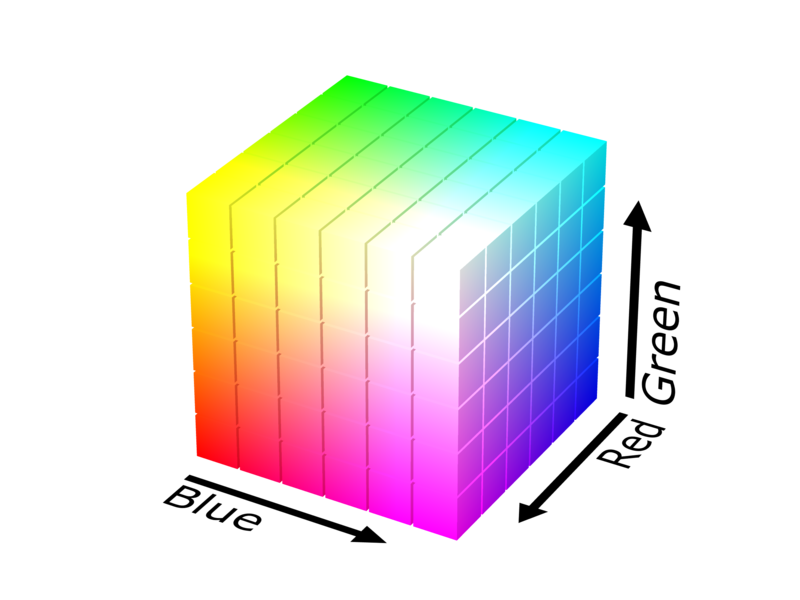
\includegraphics[height=3.3cm]{bilder/rgb.png}\label{fig:RGB}}
	\subfigure[]{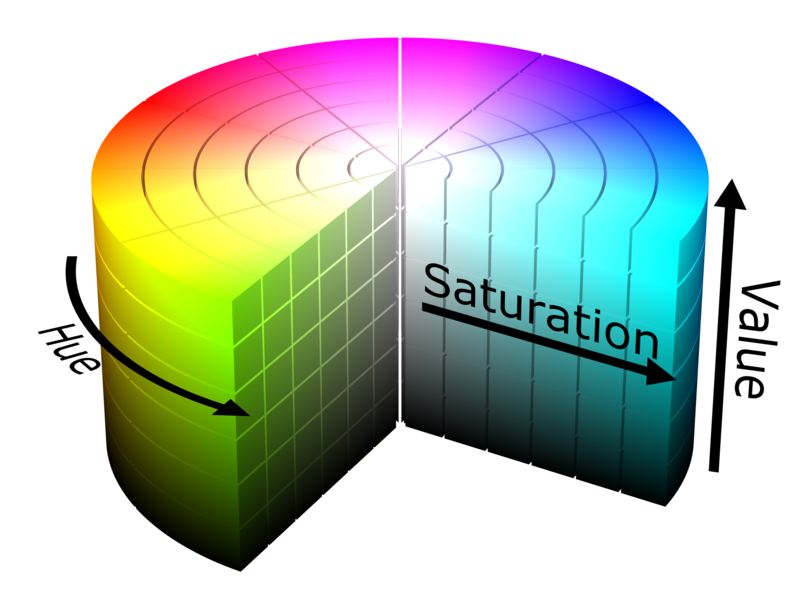
\includegraphics[height=3.0cm]{bilder/hsv.png}\label{fig:HSV}}
	\centering
	\caption{Darstellung von Farbtönen im (a) RGB-Farbraumes durch Rot-, Grün- und Blauanteileund und  im (b) HSV-Farbraumes durch Farbton (Hue), Sättigung (Saturation) und Helilgkeitswert (Value). Dunkle Farben im HSV-Farbraum haben einen kleinen Helligkeitswert.}
\end{figure}

Somit kann allein durch einen Schwellwert $\theta$ für den Helligkeitswert der schwarze Queue vom Rest des Bildes segmentiert werden.
Für das transformierte Bild $\textbf{I}_{HSV}$ ergibt sich die Berechnung des Wertes von $\textbf{B}$ an der Stelle $i, j$ für einen Schwellwert $\theta$ somit durch folgende Formel:
\begin{equation*}
\textbf{B}[i,j] = \begin{cases}
1 &\text{, falls $\textbf{I}_{HSV}[i, j, 3] \leq \theta$}\\
0 &\text{sonst}
\end{cases}
\end{equation*}

Durch die unterschiedliche Beleuchtung des Queues ergeben sich in dem entstehenden Binärbild größere Lücken, die die weitere Erkennung des Queues beeinflussen würden.
Um dies zu verhindern, werden diese durch die Anwendung eines morphologischen Closings gefüllt.
Bei einem morphologischen Closing wird zunächst eine Dilatation und daraufhin eine Erosion auf dem Bild mit einem $k \times k$ großen, ellipsoiden Fenster durchgeführt. 
Für die Dilatation wird mit dem Fenster über das Bild gelaufen und dabei der zentrale Pixel des Fensters auf den maximalen Wert im Fenster gesetzt.
Analog dazu wird bei der Erosion der Wert des zentralen Pixels auf den minimalen Wert im Fenster gesetzt.
Insgesamt werden durch diese beiden Operationen die Lücken im Binärbild geschlossen ohne die Kontur des Queues zu vergrößern.

\begin{figure}[H]
	\label{fig:thresholded}
	\subfigure[]{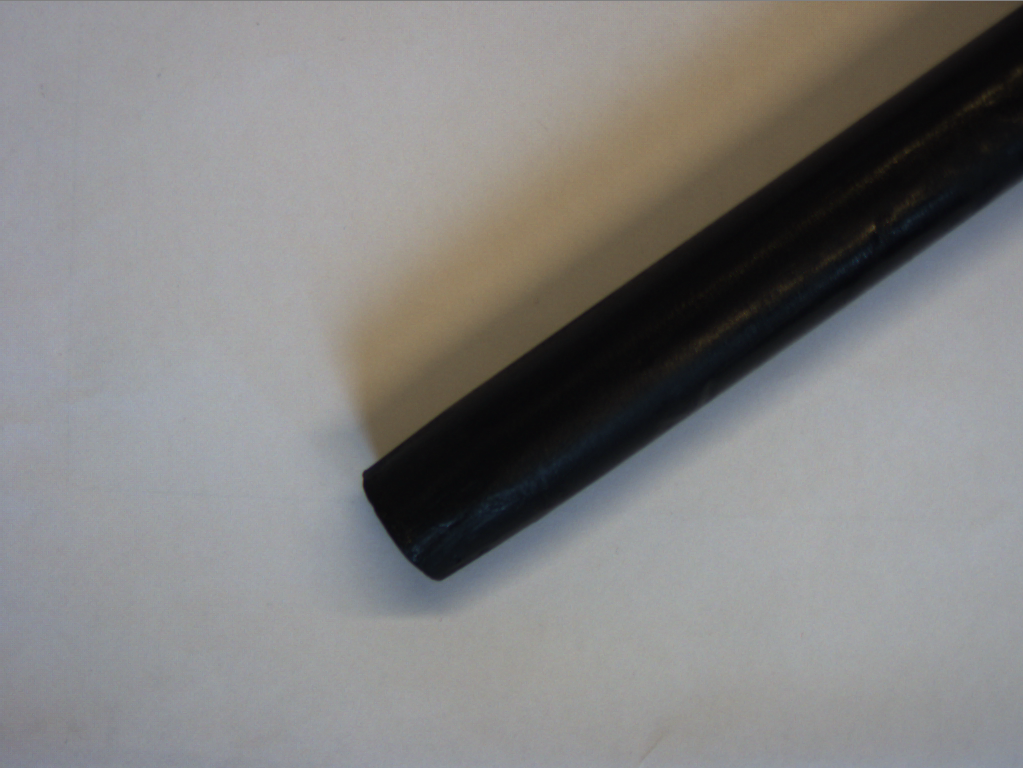
\includegraphics[height=3.3cm]{bilder/queue_orig.png}}
	\subfigure[]{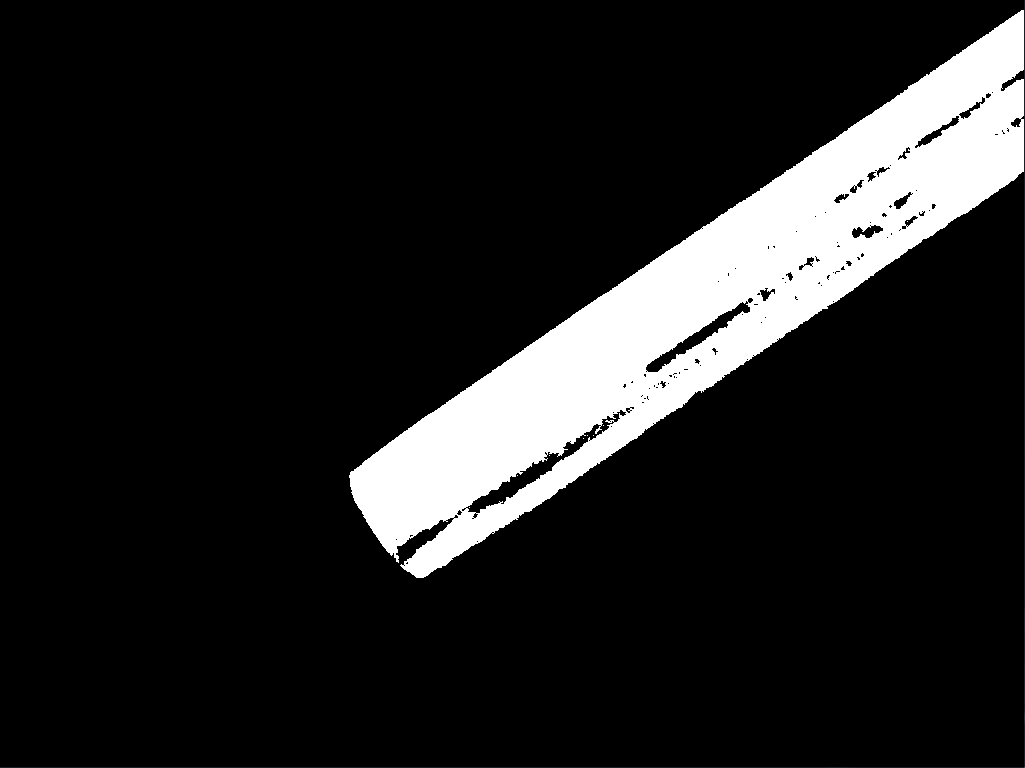
\includegraphics[height=3.3cm]{bilder/queue_thresholded.png}}
	\subfigure[]{
\includegraphics[height=3.3cm]{bilder/queue_close.png}}	
	\centering
	\caption{Ergebnis der Segmentierung des Eingabebildes. (a) Eingebild mit $1024 \times 768$ Pixeln, (b) Binärbild aus Schwellwertverfahren ($\theta = 30$),  (c) Ergebnis des morphologischen Closings ($k=9$)}
\end{figure}

\subsection{Erkennung der Queue-Enden}
Um nicht mit jedem im Binärbild als Queue klassifizierten Punkt kollidieren zu müssen, wird nur mit den Enden des Queues kollidiert.
Zur Berechnung der Position der beiden Enden wird zunächst mittels der Hauptkomponentenanalyse die Hauptachse des Queues im Bild bestimmt. 
Dazu werden zunächst die Koordinaten $i, j$ der Punkte aus $\textbf{B}$ mit $\textbf{B}[i,j] = 1$ als Zeilenvektoren in einer $n \times 2$ Matrix $\textbf{X}$ zusammengeführt.
Daraufhin werden die Mittelwerte \textbf{c} der $n$ Punkte entlang beider Dimensionen sowie die Abweichung $\textbf{A}$ zu den Mittelwerten berechnet:
\begin{equation*}
\textbf{c}[j] = \frac{1}{n}\sum_{i=1}^{n}\textbf{X}[i, j]\text{ mit }j = 1, 2
\end{equation*}
\begin{equation*}
\textbf{A} = \textbf{X} - \textbf{h}\textbf{c}^T \text{ mit } \textbf{h}[i] = 1 \text{ für } i=1,\dots,n
\end{equation*}

Aus der Matrix \textbf{A} lässt sich nun die $2 \times 2$ empirische Kovarianzmatrix $\textbf{C}$ berechnen:
\begin{equation*}
	\textbf{C} = \frac{1}{n-1}\textbf{A}^{T}\textbf{A}
\end{equation*}
Schließlich werden die zwei Eigenvektoren und Eigenwerte von $\textbf{V}$ bestimmt. 
Da der Eigenvektor $\textbf{e}$, dem der größere Eigenwert $\lambda_e$ zugeordnet ist, in die Richtung der größten Varianz der Punkte zeigt, ist die gesucht Hauptachse gegeben durch $\textbf{x}(t) = t \cdot \textbf{e} + \textbf{c}$.

Um nun die Endpunkte des Queues zu bestimmen, müssen alle Punkte auf die zuvor bestimmente Hauptachse projiziert werden.
Für einen Punkt $\textbf{x} = (i, j)$ mit $\textbf{B}[i,j] = 1$ ergeben sich folgende neue Koordinaten $\textbf{x}'$:
\begin{equation*}
	\textbf{x}' = s \cdot \textbf{e} + \textbf{c}\text{ mit } s = \frac{\textbf{e} * (\textbf{x} - \textbf{c})}{||e||_2}
\end{equation*}
Dabei bezeichnet $*$ das Skalarprodukt zweier Vektoren sowie $||\cdot||_2$ die euklidische Norm eines Vektors.
Die beiden Punkte, die am weitesten von dem Mittelpunkt \textbf{c} entfernt sind, sind die beiden Enden des Queues. Für diese Punkte $\textbf{x}_1'$, $\textbf{x}_2'$ ist $s$ entweder minimal oder maximal. 

\begin{figure}[H]
	\label{fig:thresholded}
	\subfigure[]{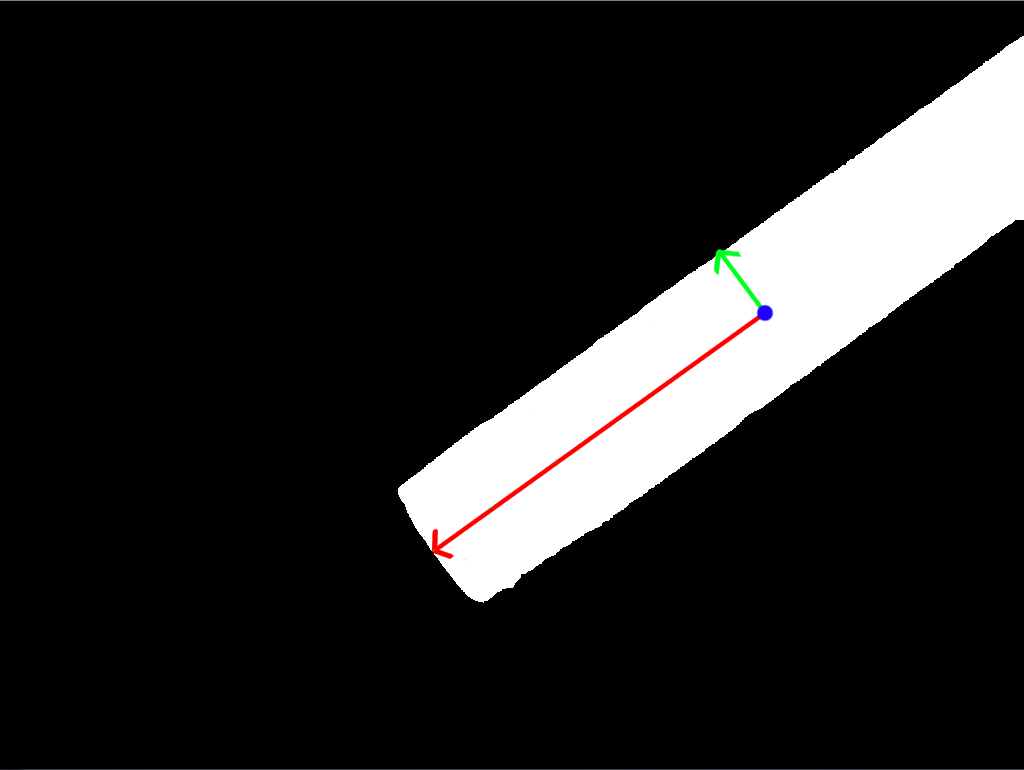
\includegraphics[height=4cm]{bilder/queue_pca_1.png}}
	\subfigure[]{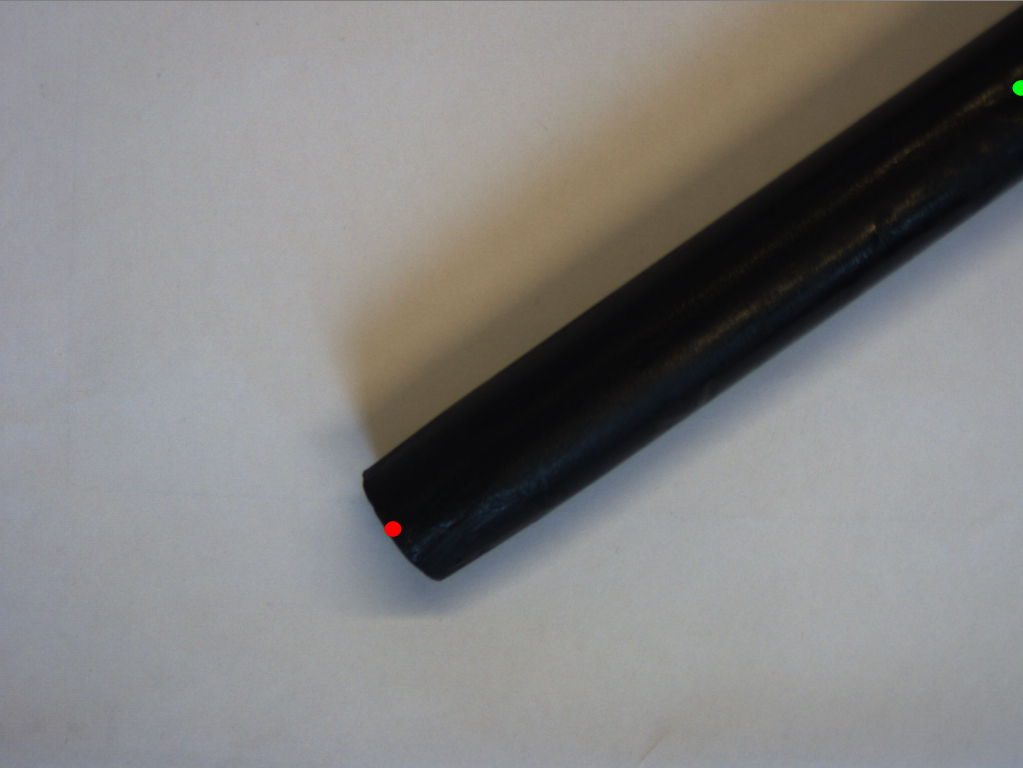
\includegraphics[height=4cm]{bilder/queue_pca_2.png}}
	\centering
	\caption{Erkannte Endpunkte des Queues. (a) Binärbild mit Zentrum \textbf{c} in blau sowie die berechneten Eigenvektoren in rot und grün, (b) Originalbild mit erkannten Endpunkten des Queues}
\end{figure}


Da das Vorzeichen für $s$ sich in aufeinanderfolgenden Bildern verändern kann, müssen die Punkte für die Kollisionsberechnung korrekt ihrem Vorgänger zugeordnet werden.
Dies wird bewerkstelligt, indem der Punkt dem näheren der beiden Vorgänger-Punkte zugeordnet wird.
Weiterhin kann keines der beiden Enden mit Sicherheit als Spitze des Queues klassifiziert werden.
Daher wird die Kollisionsbehandlung mit beiden Enden ausgeführt.
Dies hat auf den Spielfluss jedoch keine Auswirkungen, da eines der Enden meist am Rand des Spielfeldes ist.

\subsection{Kollisionserkennung}

Bei Stoßbewegungen mit dem Billard-Queue kann es zu hohen Geschwindigkeiten der Queue-Enden kommen. 
Da die Kamera mit einer Wiederholfrequenz von 25 Bildern pro Sekunde Bildaufnahmen macht, kann es passieren, dass ein Ende sich zu schnell bewegt und über eine Kugel hinwegspringt. 
Daher kann die Kollisionsüberprüfung nicht nur auf der aktuellen Position des Queue-Endes basieren.
Stattdessen wird der Kollisionspunkt durch das Schneiden der Kugel und einem  Liniensegment berechnet. 
Das Liniensegment ergibt sich dabei durch die aktuelle Position und der voherigen Position der Queue-Enden.

Die Schnittpunkte einer Kugel, gegeben durch ein Zentrum $\textbf{c}$ und Radius $r$, und einem Liniensegment, gegeben durch die Punkte $\textbf{x}^{(t)}$ und $\textbf{x}^{(t-1)}$, lässt sich wie folgt berechnen:

\hspace{-1cm}\begin{minipage}{.333333\linewidth}
	\begin{equation*}
	\textbf{d} = \textbf{x}^{(t)} - \textbf{x}^{(t-1)}
	\end{equation*}
\end{minipage}%
\begin{minipage}{.333333\linewidth}
	\begin{equation*}
	\textbf{f} = \textbf{x}^{(t-1)} - \textbf{c}
	\end{equation*}
\end{minipage}
\begin{minipage}{.333333\linewidth}
	\begin{equation*}
	s_{1,2} = \frac{-2 \cdot (\textbf{d} * \textbf{f}) \pm \sqrt{||\textbf{f}||_2^2 - r^2}}{2 \cdot ||\textbf{d}||_2^2}
	\end{equation*}
\end{minipage}



